\documentclass{article}

% Language setting
% Replace `english' with e.g. `spanish' to change the document language
\usepackage[english]{babel}

% Set page size and margins
% Replace `letterpaper' with `a4paper' for UK/EU standard size
\usepackage[letterpaper,top=2cm,bottom=2cm,left=3cm,right=3cm,marginparwidth=1.75cm]{geometry}

% Useful packages
\usepackage{amsmath}
\usepackage{graphicx}
\usepackage[colorlinks=true, allcolors=blue]{hyperref}
\usepackage{algorithm}
\usepackage{algpseudocode}
\usepackage{caption}
\usepackage{subcaption}

\usepackage{hyperref} 

\hypersetup{
    colorlinks = true,
    linkcolor=blue,
    filecolor=blue,      
    urlcolor=blue,
    citecolor=cyan,
}


\title{Programming Assignment 1}
\author{JIANJUN WEI}

\begin{document}
\maketitle


\section{Introduction}

\subsection{Description of the problem}

This project is going to find the factors that contributes to the hardest concrete. In this project, I design and implement gradient descent algorithms for uni-variate linear regression model, multi-variate linear regression model and polynomial regression model(quadratic regression model in this project) to analyze each feature and draw the conclusion.

For uni-variate linear regression model, we will follow the function
\begin{equation*}
  y=f(x)=mx+b
\end{equation*}
 where $m$ and $b$ are parameters and x is the only variable. We will calculate mean squared error in our algorithm. Also, it will be applied on our gradient descent algorithm to optimize the uni-variate linear regression model.

For multi-variate linear regression model, we will expand our input as a vector of features with length $p$. Combined with $b$ parameter, there would be $p+1$ parameters in our model. Our model could be described as 
\begin{equation*}
  y=f(x) =(m \cdot x)
\end{equation*}
, which means dot product between $m$ and $x$. In this function, $m = (m_0, m_1, \dots, m_p)^T$ and $x = (x_0, x_1, \dots, x_p)^T$. Mean squared error objective function would also be used for optimization of our linear regression model.

For polynomial regression model, we may follow the function

\begin{equation*}
   y = \MakeUppercase{X} \cdot m
\end{equation*}
where $\MakeUppercase{X}$ is a Vandermonde matrix while $m = (m_0, m_1, \dots, m_p)^T$. In this project, we would design and implement a multi-variate quadratic regression model, which means the highest order of the Vandermonde matrix $\MakeUppercase{X}$ is 2. Besides the mean squared error objective function, $R^2$ function, which represents the proportion of the variance for a dependent variable that's explained by an independent variable or variables in a regression model, would also be applied to indicate how much variation of a dependent variable is explained by the independent variable(s) in a regression model.

We will use the Concrete Compressive Strength dataset in the UCI repository\footnote{https://archive.ics.uci.edu/ml/datasets/Concrete+Compressive+Strength}. The first 900 instances would be used for training while the rest are for testing.

\subsection{Details of Algorithm}
Our algorithm is based on matrix computation. Although our gradient descent algorithm is not stochastic, we still get much greater training and testing results. 

For uni-variate linear regression model, we set the initial learning rate 0.00001. Since one independent feature may have much larger impact on the observed output, we set a smaller learning rate so that it could be slowly descended without missing the local minimum. However, when training multi-variate and polynomial regression model, the initial learning rate we choose is 0.0001. The reason why it is a little larger than the uni-variate linear regression model is that these two models take all features into consideration, which means that they will have less impact on the output observed data. Thus, we could learning a little bit fast than the uni-variate regression model. The learning rate is adaptive in our algorithm when we train the data. We adjust it according the difference between the value of two mean squared error(MSE). When the new MSE is less than the previous one, we would accelerate our training process by setting it into 120 percent of its original value. Otherwise, we set it into 75 percent since the difference between the new MSE and the previous one now is a signal that we are moving too fast.

For all three models, we set the max steps as 100000. When the difference of the two MSE is less than 1e-18, or we have already moved 100000 steps, we will stop training since the loss function is approaching convergence in this situation and would not have too much change later. 

Since our algorithm is based on matrix computation, the derivative equation might be slightly different from we have learnt in class. They actually have the same meaning, but different in representation. Our derivative equation will be:
\begin{equation*}
  \frac{\partial J}{\partial M} = (M^T X^T X - y ^TX)
\end{equation*}
where $M = (m_0, m_1, \dots, m_p)$. And thus, we will update the parameters according to the following function:
\begin{equation*}
  M_{k+1} = M_k - \alpha  \frac{\partial J}{\partial M}
\end{equation*}

\subsection{Pseudo-code of algorithm}
Here is the pseudo-code of descend gradient algorithm:
\begin{algorithm}
\caption{Pseudo-code of our descend gradient algorithm}\label{alg:cap}
\begin{algorithmic}
\Require $training input, parameter, training output, learning rate, max step$

\State size $ \gets $ count of training data
\State previous loss $\gets Inf$
\State diff $ \gets Inf$
\State $step \gets 0 $

\While{diff $\textgreater$  1e-18 and max step $\textless$ 100000}

\State calculate derivative matrix

\State update parameter matrix $M$

\State calculate loss function MSE

\State calculate difference between previous MSE and the new one

\State adjust learning rate according to the previous MSE and the new one

\State $step \gets step + 1 $

\State set previous loss

\EndWhile
\end{algorithmic}
\end{algorithm}


The following part will be the whole process of optimized regression model algorithm:

\begin{algorithm}
\caption{Pseudo-code of optimized regression model algorithm}\label{alg:cap}
\begin{algorithmic}
\Require dataset

\State Splitting data into training set and testing set
\State Pre-processing training set

\If{uni-variate linear regression}

    \State training model for each features
    \State testing model according to training results
    
\ElsIf{multi-variate linear regression}
    \State training model for multi-variate linear regression
    \State testing model according to training results
\ElsIf{polynomial regression}
    \State training model for polynomial regression
    \State testing model according to training results
\EndIf

\end{algorithmic}
\end{algorithm}


\subsection{Normalize the data}
We would like to normalize our input data in our all three regression models. Since the output would only be influenced by single variable in uni-variate linear regression, there would be just slightly difference after normalization. However, when dealing with multiple variables, the features have different units and they all contribute to the output data. Thus, we need to normalize all the features to avoid the situation that the output will be over dependent on one or some features.

In this project, we would like to normalize each feature as the following function:
\begin{equation*}
  x\_norm = \frac{x - \mu}{s}
\end{equation*}
where $\mu$ is the mean of the feature and $s$ is the standard deviation.

Figure \ref{fig:no_norm} and Figure \ref{fig:norm} are the histograms that illustrate how the distribution of a feature variable’s values changed. In Figure \ref{fig:no_norm}, we do not pre-processing the data and we could see the range of the value would be [0, 1200]. However, after we normalize the input data, we could see in Figure \ref{fig:norm} that the range comes to [-3, 5], which would be much more helpful to grasp the real features and train the correct and useful model.


\begin{figure}[htbp]
    \centering
    \begin{minipage}[t]{0.49\textwidth}
        \centering
        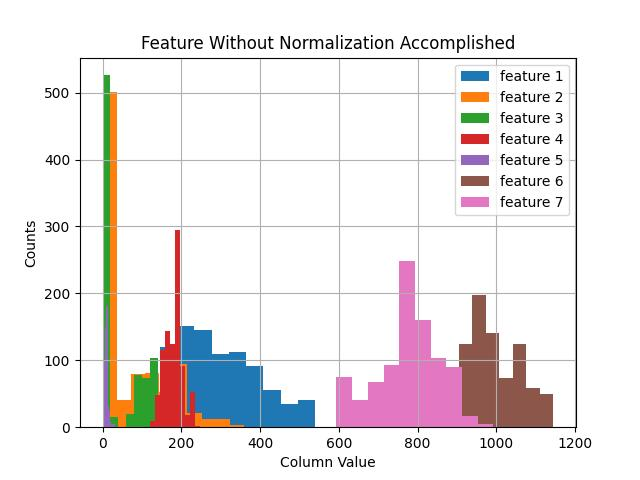
\includegraphics[width=7.7cm]{images/without_norm.jpg}
        \caption{Data without normalization}
        \label{fig:no_norm}
    \end{minipage}
    \begin{minipage}[t]{0.49\textwidth}
        \centering
        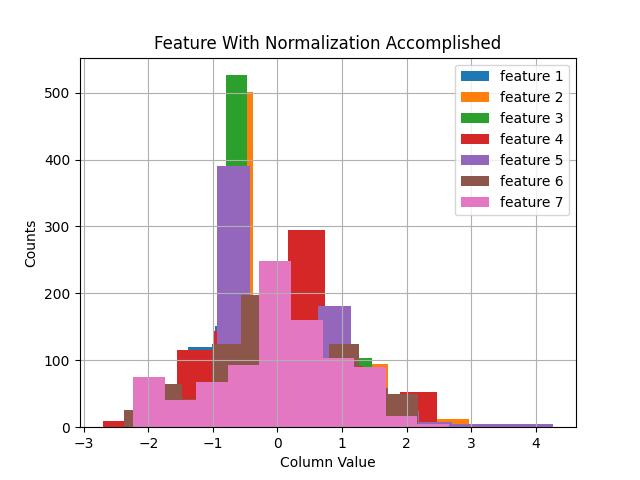
\includegraphics[width=7.7cm]{images/with_norm.jpg}
        \caption{Data with normalization}
        \label{fig:norm}
    \end{minipage}
\end{figure}



\begin{table}[htbp]
\centering
\begin{tabular}{|l|c|c|c|c|}
\hline
Feature & MSE(norm) & R\_square(norm) & MSE( without norm) & R\_square( without norm)\\
\hline
Cement & 241.214 & 0.185 & 241.216 & 0.185\\
\hline
Blast Furnace Slag & 290.773 & 0.0172  & 290.773 & 0.0172\\
\hline
Fly Ash & 295.262 & 0.002  & 295.262 & 0.002 \\
\hline
Water  & 343.997 & -0.162 & 344.001 & -0.162\\
\hline
Superplasticizer & 244.301 & 0.174 & 244.301 & 0.174\\
\hline
Coarse Aggregate  & 322.252 & -0.0891 & 322.252 & -0.089\\
\hline
Fine Aggregate &  333.095 & -0.125 & 333.095 & -0.125\\
\hline
Age  & 262.910 & 0.111 & 262.910 &  0.111 \\

 
\hline
\end{tabular}
\caption{\label{tab:train_uni}Results for uni-variate linear regression model on training data set.}
\end{table}


\section{Results}
In this section, we put much more emphasis on the results. Here we may focus on the "R\_square", which could be defined as:

\begin{equation*}
  1 - \frac{MSE}{Variance(observed)}
\end{equation*}


\subsection{Variance explained of models on the training data set}

For uni-variate linear regression model, the result has shown in Table \ref{tab:train_uni}.



For multi-variate linear regression model, the result has shown in Table \ref{tab:train_multi}. We have already normalized the training data set.

\begin{table}[htbp]
\centering
\begin{tabular}{|l|c|c|}
\hline
         &  MSE & R\_square \\
\hline
with norm &  115.051  & 0.611 \\
\hline
without norm & 114.629 & 0.612 \\
\hline
\end{tabular}
\caption{\label{tab:train_multi}Results for multi-variate linear regression model on training data set.}
\end{table}





For polynomial regression model, the result has shown in Table \ref{tab:train_poly}. Also, we have already normalized the training data set and more precisely, in this project we mainly focus on the quadratic regression model.

\begin{table}[htbp]
\centering
\begin{tabular}{|l|c|c|}
\hline
         &  MSE & R\_square \\
\hline
with norm &  56.584  & 0.808 \\
\hline
without norm & 55860.771 & -187.805 \\
\hline
\end{tabular}
\caption{\label{tab:train_poly}Results for multi-variate quadratic regression model on training data set.}
\end{table}








\subsection{Variance explained of models on the testing data set}

For uni-variate linear regression model, the result has shown in Table \ref{tab:test_uni}.


\begin{table}[htbp]
\centering
\begin{tabular}{|l|c|c|c|c|}
\hline
Feature & MSE(with norm) & R\_square(with norm)& MSE(without norm) & R\_square(without norm)\\
\hline
Cement & 98.996 & 0.311 & 99.313 & 0.308\\
\hline
Blast Furnace Slag & 159.685 & -0.111 & 159.687 & -0.111\\
\hline
Fly Ash & 149.467 & -0.039 & 149.480 & -0.040\\
\hline
Water  & 179.496 & -0.248 & 179.599 & -0.249\\
\hline
Superplasticizer & 235.338 & -0.637 & 235.338 & -0.637\\
\hline
Coarse Aggregate  & 165.900 & -0.154 & 165.900 & -0.154\\
\hline
Fine Aggregate & 171.355 & -0.192 & 171.346 & -0.192\\
\hline
Age  & 150.919 & -0.050 & 150.924 & -0.050\\
\hline
\end{tabular}
\caption{\label{tab:test_uni}Results for uni-variate linear regression model on training data set.}
\end{table}








For multi-variate linear regression model, the result has shown in Table \ref{tab:test_multi}. In addition, the testing data set has already been normalized.

\begin{table}[!ht]
\centering
\begin{tabular}{|l|c|c|}
\hline
         &  MSE & R\_square \\
\hline
with norm &  64.393  & 0.551\\
\hline
without norm & 60.07 & 0.582 \\
\hline
\end{tabular}
\caption{\label{tab:test_multi}Results for multi-variate linear regression model on testing data set.}
\end{table}





For polynomial regression model, the result has shown in Table \ref{tab:test_poly}. Also, the testing data set is normalized. And, more precisely, in this project we mainly focus on the quadratic regression model.

\begin{table}[!ht]
\centering
\begin{tabular}{|l|c|c|}
\hline
         &  MSE & R\_square \\
\hline
with norm &  46.565  & 0.675\\
\hline
without norm & 105424.342 & -732.543 \\
\hline
\end{tabular}
\caption{\label{tab:test_poly}Results for multi-variate quadratic regression model on testing data set.}
\end{table}




\subsection{Plots of uni-variate models }
Figure \ref{fig:0} to Figure \ref{fig:7} show the images of uni-variate models. The trained uni-variate models are printed on top of scatter plots of the training data used.

\begin{figure}[!htbp]
    \centering
    \begin{minipage}[t]{0.49\textwidth}
        \centering
        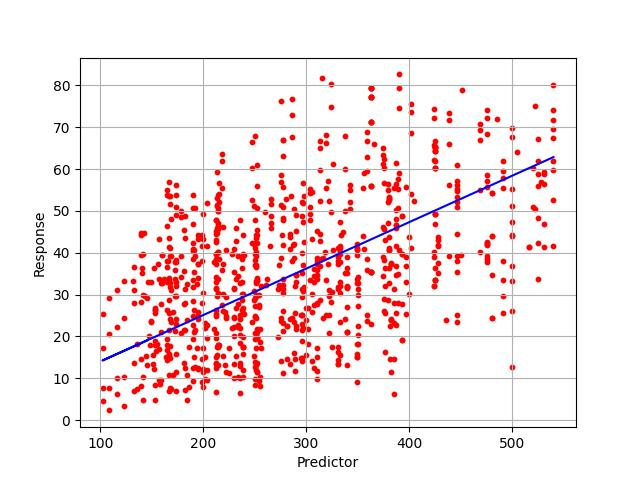
\includegraphics[height = 5.6cm, width=6.6cm]{images/0.jpg}
        \caption{Feature: Cement, uni-variate linear regression}
        \label{fig:0}
    \end{minipage}
    \begin{minipage}[t]{0.49\textwidth}
        \centering
        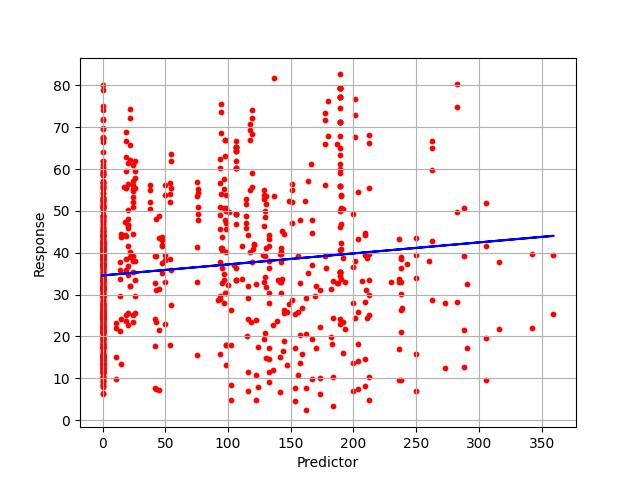
\includegraphics[height = 5.6cm, width=6.6cm]{images/1.jpg}
        \caption{Feature: Blast Furnace Slag, uni-variate linear regression}
        \label{fig:1}
    \end{minipage}
\end{figure}

\begin{figure}[!htbp]
    \centering
    \begin{minipage}[t]{0.49\textwidth}
        \centering
        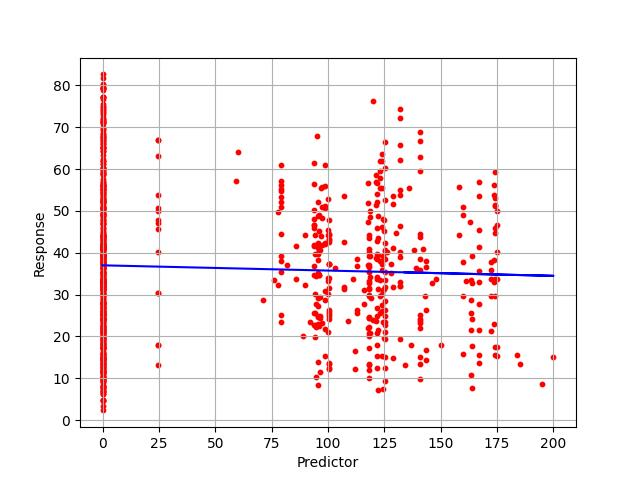
\includegraphics[height = 5.6cm, width=6.6cm]{images/2.jpg}
        \caption{Feature: Fly Ash, uni-variate linear regression}
        \label{fig:2}
    \end{minipage}
    \begin{minipage}[t]{0.49\textwidth}
        \centering
        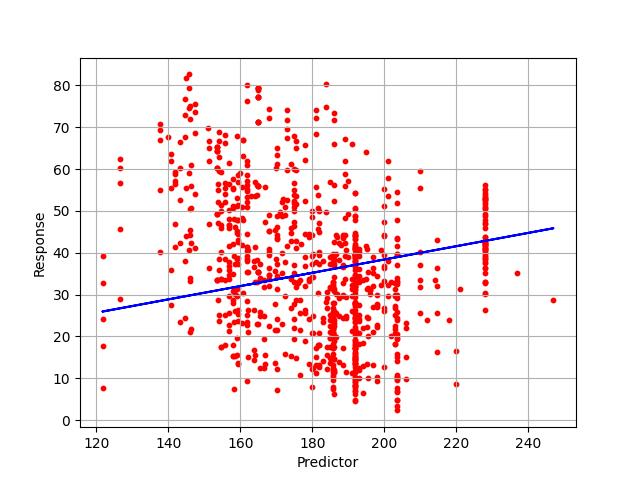
\includegraphics[height = 5.6cm, width=6.6cm]{images/3.jpg}
        \caption{Feature: Water, uni-variate linear regression}
        \label{fig:3}
    \end{minipage}
\end{figure}


\begin{figure}[!h]
    \centering
    \begin{minipage}[t]{0.49\textwidth}
        \centering
        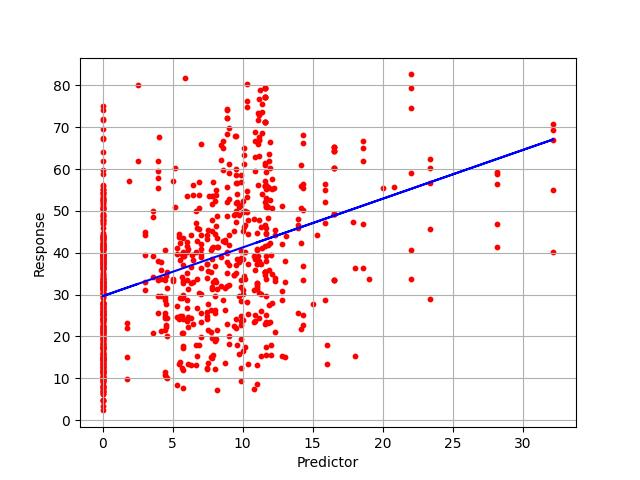
\includegraphics[height = 5.6cm, width=6.6cm]{images/4.jpg}
        \caption{Feature: Superplasticizer, uni-variate linear regression}
        \label{fig:4}
    \end{minipage}
    \begin{minipage}[t]{0.49\textwidth}
        \centering
        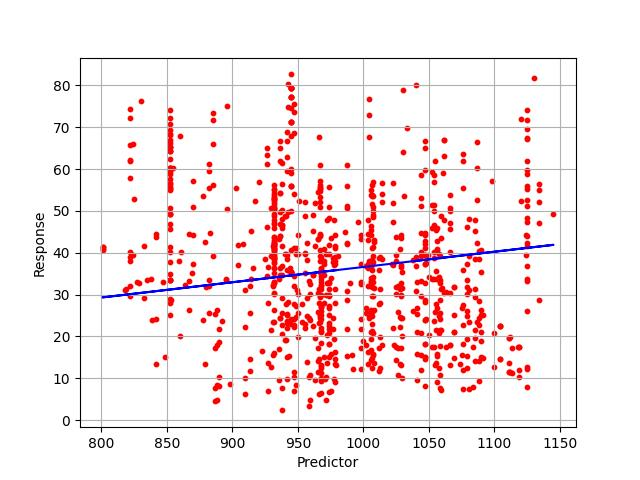
\includegraphics[height = 5.6cm, width=6.6cm]{images/5.jpg}
        \caption{Feature: Coarse Aggregate, uni-variate linear regression}
        \label{fig:5}
    \end{minipage}
\end{figure}


\begin{figure}[!h]
    \centering
    \begin{minipage}[t]{0.49\textwidth}
        \centering
        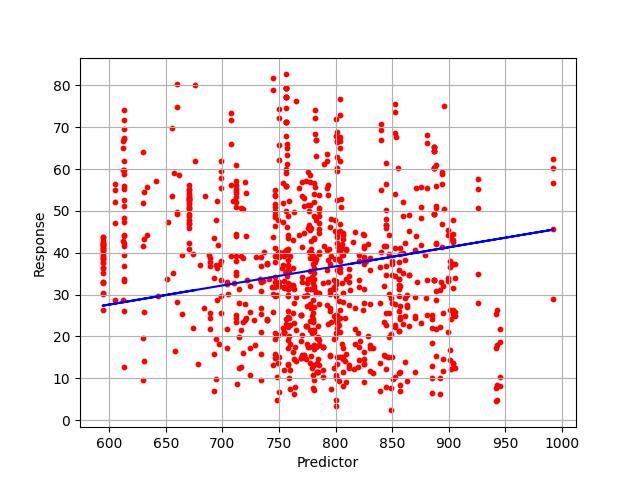
\includegraphics[height = 5.6cm, width=6.6cm]{images/6.jpg}
        \caption{Feature: Fine Aggregate, uni-variate linear regression}
        \label{fig:6}
    \end{minipage}
    \begin{minipage}[t]{0.49\textwidth}
        \centering
        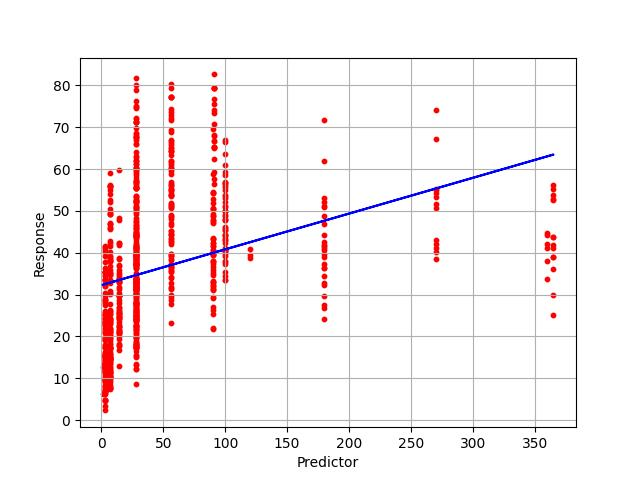
\includegraphics[height = 5.6cm, width=6.6cm]{images/7.jpg}
        \caption{Feature: Age, uni-variate linear regression}
        \label{fig:7}
    \end{minipage}
\end{figure}







\section{Discussion}

\subsection{Describe models compared in performance on the training data}
We have trained the data set from three models, the uni-variate linear regression model, the multi-variate linear regression model and quadratic regression model. They all have different performance.

From the result, we could see that quadratic model gets much lower loss function and much higher R\_square value compared to the linear regression. The reason may lie in the fact that quadratic model has much more complex function which allows it to learn or match the features we provide. However, although the multi-variate linear regression model takes all features into consideration, the model did not take care the high dimensional data, which means the model could not learn features with high dimension well. For uni-variate model, since it only consider one variable a time, it performs not as good as multi-variate regression model and quadratic model.

For all three models we choose in this project, the coefficients trained from the training data points performs well on testing data, but the result of testing data is a little bit different from the result of training data. One of the reason is that we have 900 data for training but 130 data for testing. When we have more data, regardless of training data or testing data, our model could have more chance to learn feature. As a result, we could get much more precise coefficient and performance would be improved.



\subsection{Describe the coefficients of the uni-variate models}
We could know that the coefficients of the uni-variate models fail to predict the coefficients in the multi-variate model. 

In uni-variate regression model, we separate all features into individual one. It is true that the model learns the influence from each feature to the output data, but they are independent and we did not take the combination of these features into consideration. This means that we ignore some features that we should have learned. As a result, the coefficients of the uni-variate models did not perform well when predict the coefficients in the multi-variate model.


\subsection{Draw some conclusions about what factors predict concrete compressive strength}
We could know from the project the the more correct data we have, the higher possibility that could be to help us precisely predict the concrete compressive strength. In addition, a powerful model also contributes to the prediction of the result. A powerful model means that the model has a much more powerful learning ability that could be adaptive to more complex data input and various features. Besides, chosing the suitable learning rate and normalization function would be speed up the training process and improve the training results.

From my point of view, it is the cement, water, blast furnace slag and fine aggregate that contributes to the hardest possible concrete. So when we hope to make the concrete, we may put more emphasis on these ingredients so that we could make a much harder concrete.


\subsection{Comparisons to the results from normalized}
Usually, we normalize the training data points when we need to take several features into consideration. We could see from the histogram in the previous section and find that the range of the data is much larger and the value of every feature vary from each other. When we start regression without data normalization, the value of each feature will be larger especially when we combine several feature together. And the result is that we get a huge MSE when we start training and need to take a much longer path to descend the gradient to get the parameters we need, which will take much more time to grasp the feature that really contributes to the hardest concrete.

We could see that although the results with normalization and the those without normalization in our uni-variate and multi-variate linear regression model are similar, there is a huge difference in our quadratic model. The reason is that we have already do enough steps for data without normalization in our first 2 models and they reach out the condition that could hardly descend in gradient, however, since the quadratic model is much more complex, the max steps for first two model is not satisfied and we need a much smaller learning rate and more steps to train the data so that the loss function could become much more flat.

In addition, when we normalize the data, we limit the range of all features in a much smaller value. This may help us quickly find the correct and proper parameter that satisfy the training data and features since data now is more concentrated and we have a much shorter descend path when we running descend gradient algorithm.


\section{Code}
This project is written in Python. The input data is the CSV file which contains all the data we need. The output will be the images we may need to be used to analyze and some metrics that we calculated.

By setting the correct path of the input CSV file, the program could be run just by a simple click of mouse.

\subsection{Source Code}
For the source code, I have already updated on the github. You could get the code as well as the data set from \url{https://github.com/weijj27/514-Programming-Assignment}.

%\bibliographystyle{alpha}
%\bibliography{sample}

\end{document}